\chapter{Results and Discussion}\label{chap:results_discussion}
\section{Binary Classification}
\subsection{Metrics}
When assessing the performance of a binary prediction model using a validation dataset containing known target values, four key metrics come into play:

\begin{itemize}
  \item True Positives (TP): The number of correctly predicted active cases.
  \item True Negatives (TN): The number of correctly predicted inactive cases.
  \item False Positives (FP): The number of incorrectly predicted active cases.
  \item False Negatives (FN): The number of incorrectly predicted inactive cases.
\end{itemize}


Using these four values, it is possible to construct a confusion matrix, as illustrated in Table~\ref{tab:confusion_matrix}.

\begin{table}[h]
  \centering
  \caption{Confusion Matrix}
  \label{tab:confusion_matrix}
  \setlength{\tabcolsep}{10pt} % Adjust cell padding
  \renewcommand{\arraystretch}{1.5} % Adjust cell height
  \begin{tabular}{|c|c|c|}
  \cline{2-3}
  \multicolumn{1}{c|}{} & Actual Negative & Actual Positive \\
  \hline
  Predicted Negative & TN & FN \\
  \hline
  Predicted Positive & FP & TP \\
  \hline
  \end{tabular}
\end{table}

In binary classification, the classification threshold is a crucial parameter dictating how the model assigns data points to one of two classes based on predicted probabilities or scores. This threshold significantly influences the model's metrics, as illustrated in Figure~\ref{fig:classification_threshold}.
\begin{figure} 
  \centering
  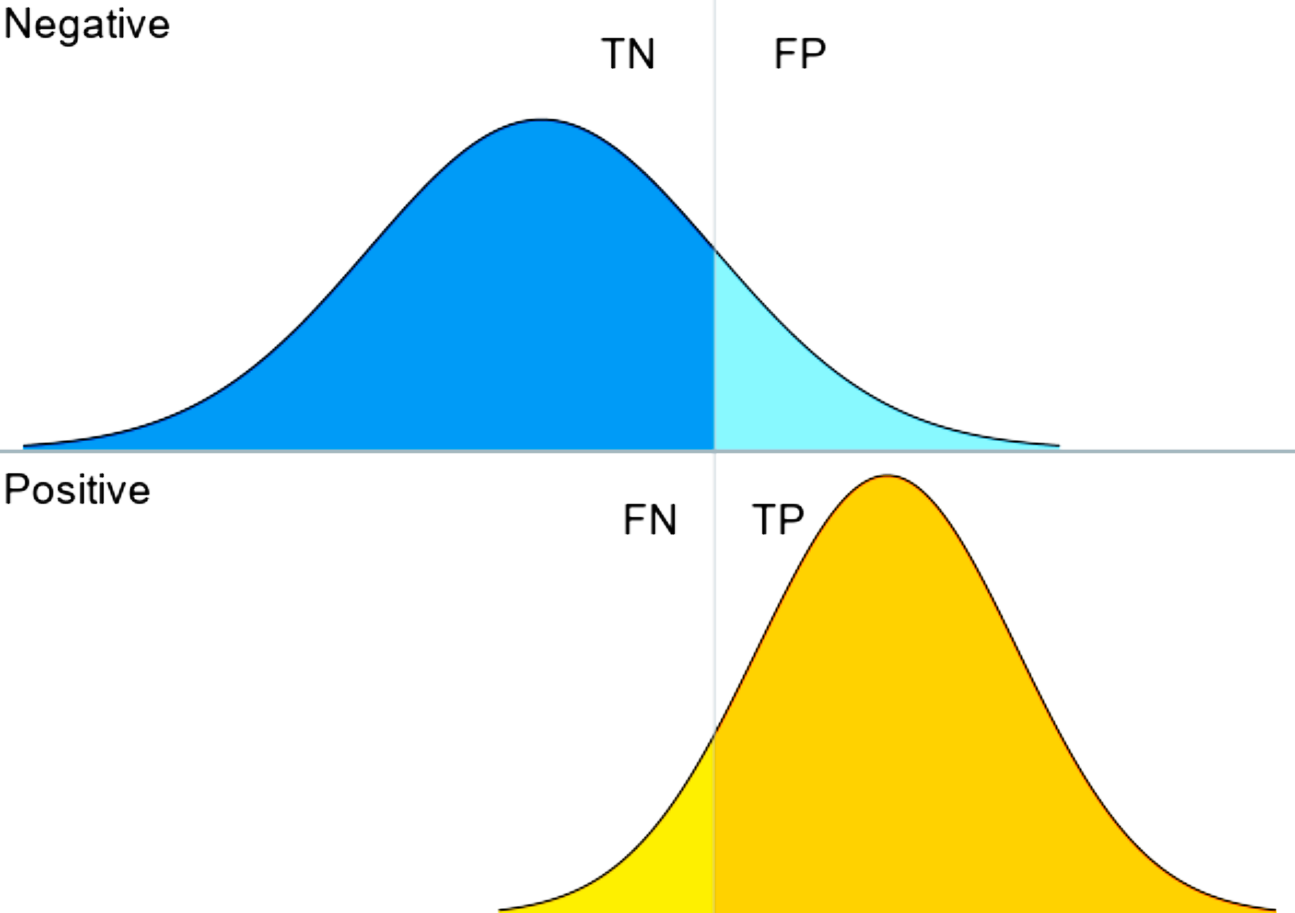
\includegraphics[width=0.5\textwidth]{figures/classification_threshold.png}
  \caption{Relationship between threshold and classification. Figure obtained from~\cite{wicklin2020}}
~\label{fig:classification_threshold}
\end{figure}

Several evaluation metrics can help assess the performance of a predictive model. These metrics include:

\begin{itemize}
  \item \textbf{Accuracy}: The ratio of correctly classified instances (TP) and (TN) to the total number of instances. It provides a general measure of the model's correctness.
  \[ \text{Accuracy}  A = \frac{TP + TN}{TP + TN + FP + FN} \]

  \item \textbf{Precision (P)}: The proportion of correctly predicted active cases (TP) to all instances predicted as active (TP + FP). 
  \[ \text{Precision } P = \frac{TP}{TP + FP} \]

  \item \textbf{Recall (R) or Sensitivity or True Positive Rate (TPR)}: The proportion of correctly predicted active cases (TP) to all actual active cases (TP + FN).
  \[ \text{Recall } R = \frac{TP}{TP + FN} \]

  \item \textbf{F1 Score}: The harmonic mean of precision and recall, which balances the trade-off between false positives and false negatives.
  \[ F1 = \frac{2 \cdot P \cdot R}{P + R} \]

  \item \textbf{True Negative Rate (TNR) Specificity}: The proportion of correctly predicted inactive cases (TN) to all actual inactive cases (TN + FP).
  \[ TNR = \frac{TN}{TN + FP} \]

  \item \textbf{Receiver Operating Characteristic (ROC) Curve}: A graphical representation of the model's performance across different classification thresholds. It plots the true positive rate (TNR) against the false positive rate (FPR).
  
\end{itemize}


\subsubsection{Imbalanced Data}
Exemplified in Figure~\ref{fig:confusion_matrix}, the majority of assay endpoints exhibit an imbalance in the distribution of active (positive) and inactive (negative) compounds when employing binarized toxicity hitcalls. Mostly the negative class significantly outweighs the postive class. Imbalanced datasets can lead to skewed performance metrics, as the model may perform well on the majority class but poorly on the minority class. To address imbalanced datasets, additional metrics such as macro-averaged and weighted-averaged metrics can be taken into account.
\begin{figure}[h]
  \centering
  \includegraphics[width=0.7\textwidth]{figures/roc97.png}
  \caption{For assay endpoint with aeid: 97, the Receiver Operating Characteristic (ROC) curve is shown for the XGBoost Classifier. We predicted each trained model with four different classification thresholds, namely default = 0.5, optimal = cost(TPR, FPR), True Positive Rate = 0.5 (tnr), True Negative Rate = 0.5 (tnr).}
~\label{fig:confusion_matrix}
\end{figure}


\begin{figure} 
  \centering
  \includegraphics[width=1.0\textwidth]{figures/cm97.png}
  \caption{For assay endpoint with aeid: 97, confusion matrices are shown for four different classification thresholds.}
~\label{fig:confusion_matrix}
\end{figure}

The majority of assay endpoints exhibit an imbalance in the distribution of active (positive) and inactive (negative) compounds when employing binarized toxicity hitcalls. Mostly the negative class significantly outweighs the postive class. Imbalanced datasets can lead to skewed performance metrics, as the model may perform well on the majority class but poorly on the minority class. To address imbalanced datasets, additional metrics such as macro-averaged and weighted-averaged metrics can be taken into account.

In macro-averaging, the metric is computed separately for each class, and then an unweighted average is taken. This approach assigns equal importance to each class, regardless of their representation within the dataset. As an example, macro-averaged precision calculates the unweighted average of precision across all classes, whereas the weighted-average of precision considers the impact of class prevalence.
\[ \text{Macro-Precision } = \frac{1}{N} \sum_{i=1}^{N} P_i \] 
\[ \text{Weighted-Precision } = \frac{1}{N} \sum_{i=1}^{N} \left(\frac{TP_i}{TP_i + FP_i}\right) \cdot \frac{N_i}{N} \]

In both cases, $N$ is the total number of classes (e.g. $N=2$ for the binary case), and $N_i$ represents the number of samples in class $i$. Similarly the macro-averaged and weighted-averaged recall and F1 score can be calculated.



\subsection{Performance}
We evaluated the model performance using the previously mentioned metrics. The following figures show the performance metrics applied to:

\begin{enumerate}
  \item the internal validation dataset (Figure~\ref{fig:hitcall_classification_xgb_val_default_macro_avg},~\ref{fig:hitcall_classification_xgb_val_default_weighted_avg},~\ref{fig:hitcall_classification_xgb_val_default_true},~\ref{fig:hitcall_classification_xgb_val_default_false})
  \item the fingerprint from the MassBank structure validation set (\ref{fig:hitcall_classification_xgb_val_default_macro_avg},~\ref{fig:hitcall_classification_xgb_val_default_weighted_avg},~\ref{fig:hitcall_classification_xgb_val_default_true},~\ref{fig:hitcall_classification_xgb_val_default_false})
  \item the SIRIUS-predicted fingerprint from the MassBank validation set (\ref{fig:hitcall_classification_xgb_val_default_macro_avg},~\ref{fig:hitcall_classification_xgb_val_default_weighted_avg},~\ref{fig:hitcall_classification_xgb_val_default_true},~\ref{fig:hitcall_classification_xgb_val_default_false})
\end{enumerate}

For each validation set, four figures are presented, each of which shows a different perspective on the performance metrics:

\begin{enumerate}
  \item the \emph{macro average} metrics
  \item the \emph{weighted average} metrics
  \item the separately sliced metrics for the \emph{positive} class
  \item the separately sliced metrics for the \emph{negative} class
\end{enumerate}

The default classification threshold, which is 0.5, was used for predicting the class labels. Each figure shows performance on the binarized hitcall without cytotoxicity correction, in a scatter plot that compares precision against recall for all target assay endpoints employing each of the classifiers. All models use an XGBoost classifier as the underlying feature selection model. The marker size in the scatter plots reflects the varying number of compounds in the validation set across the assay endpoints. The marginal boxplots illustrate the distribution of the performance metrics across the target assay endpoint models. The adjacent table provides the average metrics for the estimators across all target assay endpoint models.


\subsubsection{Internal validation}
\begin{figure}[h]
  \centering
  \includegraphics[width=0.99\textwidth]{figures/hitcall_classification_xgb_val_default_macro_avg.png}
  \caption{}
~\label{fig:hitcall_classification_xgb_val_default_macro_avg}
\end{figure}

\begin{figure}[h]
  \centering
  \includegraphics[width=0.99\textwidth]{figures/hitcall_classification_xgb_val_default_weighted_avg.png}
  \caption{}
~\label{fig:hitcall_classification_xgb_val_default_weighted_avg}
\end{figure}

\begin{figure}[h]
  \centering
  \includegraphics[width=0.99\textwidth]{figures/hitcall_classification_xgb_val_default_true.png}
  \caption{}
~\label{fig:hitcall_classification_xgb_val_default_true}
\end{figure}

\begin{figure}[h]
  \centering
  \includegraphics[width=0.99\textwidth]{figures/hitcall_classification_xgb_val_default_false.png}
  \caption{}
~\label{fig:hitcall_classification_xgb_val_default_false}
\end{figure}

\subsubsection{MassBank structure validation}
\begin{figure}[h]
  \centering
  \includegraphics[width=0.99\textwidth]{figures/hitcall_classification_xgb_val_default_macro_avg.png}
  \caption{}
  ~\label{fig:hitcall_classification_xgb_val_default_false}
\end{figure}


Perfromance results were generated for every combination of the three validation sets, the two target variables (hitcall, cytotoxicity corrected hitcall),  $\geq 300$ assay endpoints, two feature selection models (XGBoost, RandomForest), four classiifaction thresholds (default, optimal, TPR=0.5, TNR=0.5). 